\begin{problem}{관악산 등산}{standard input}{standard output}

서울대학교에는 ``누가 조국의 미래를 묻거든 고개를 들어 관악을 보게 하라''라는 유명한 문구가 있다. 어느 날 Unused는 Corea에게 조국의 미래를 물었고, Corea는 직접 관악산에 올라가 조국의 미래를 보고 답해 주기로 했다.

관악산의 등산로는 $1$부터 $N$까지의 서로 다른 번호가 붙어 있는 $N$개의 쉼터와 두 쉼터 사이를 오고갈 수 있는 $M$개의 길들로 이루어져 있다. Corea는 지면에서부터 산을 올라가는 것은 너무 귀찮다고 생각했기 때문에, 케이블카를 타고 임의의 쉼터에서 내린 다음 등산을 시작하기로 했다. 심지어 등산로 지도를 보는 것도 귀찮았던 Corea는 지금 있는 쉼터와 길 하나로 연결되어 있으면서 지금보다 더 높은 곳에 있는 쉼터를 하나 골라서 올라가는 것을 반복하면 산의 정상에 도착할 수 있을 거라고 생각했다. 물론 실제로는 그렇지 않을 수도 있다.

Corea가 임의의 쉼터에서 출발하여 자신의 생각에 따라 산을 오를 때, 최대 몇 개의 쉼터를 방문할 수 있는지 구하여라.

\InputFile
첫 번째 줄에 등산로에 있는 쉼터의 수 $N$($1 \le N \le 3000$)과 두 쉼터 사이를 연결하는 길의 수 $M$($1 \le M \le 50,000$)이 주어진다.

두 번째 줄에는 각 쉼터의 높이를 나타내는 $N$개의 정수가 번호 순서대로 주어진다. 각 쉼터의 높이는 $1$ 이상 $1,000,000$ 이하이며 서로 다르다.

세 번째 줄부터 $M$개의 줄에 걸쳐 각각의 길이 연결하는 두 쉼터의 번호가 공백으로 구분되어 주어진다. 쉼터의 번호는 $1$ 이상 $N$ 이하의 정수이다. 양 끝점이 같은 쉼터인 길은 없으며, 임의의 두 쉼터를 연결하는 길이 여러 개 존재할 수 있다.

\OutputFile
Corea가 각 쉼터에서 출발할 때 최대로 방문할 수 있는 쉼터의 개수를 번호 순서대로 한 줄에 하나씩 $N$줄에 걸쳐 출력한다.

\Example

\begin{example}
\exmp{5 5
3 1 6 4 7
1 4
2 1
3 4
4 2
5 1}{3
4
1
2
1}%
\end{example}

\Notes
\begin{center}
  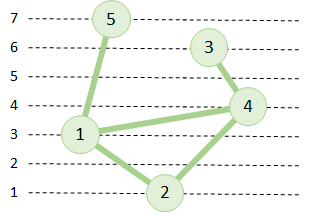
\includegraphics[width=0.4\textwidth]{climb.png}
\end{center}

2번 쉼터에서 출발하면 1번, 4번, 3번 쉼터를 차례대로 방문할 때 가장 많은 쉼터를 방문할 수 있다.

5번 쉼터는 3번 쉼터보다 높은 곳에 있지만 길 하나로 연결되어 있지 않으므로 3번 쉼터에서 5번 쉼터로 이동할 수 없다.

\end{problem}
